
\subsection{Forza di Attrito Radente}
L'attrito radente è una forza che si manifesta tra due superfici a contatto e scabre, opponendosi al loro moto relativo (o alla tendenza al moto).

\subsubsection{Attrito Statico ($F_s$)}
È la forza parallela alla superficie presente quando il corpo è \textbf{fermo} su una superficie scabra. Essa \textbf{si oppone} alla risultante delle forze parallele che tenderebbero a muovere il corpo.
\begin{itemize}
    \item Se non c'è alcuna forza parallela applicata, l'attrito è nullo ($\sum F_{\parallel} = 0 \Rightarrow F_s = 0$).
    \item L'attrito statico è una forza "intelligente": cresce in modulo per bilanciare esattamente la forza esterna applicata, fino a un valore limite massimo.
\end{itemize}

\begin{equation}
    |\vec{F}_s| \le \mu_s |\vec{N}|
\end{equation}

Il valore massimo (limite di rottura dell'equilibrio) è:
\[ F_{s,max} = \mu_s N \]
Questa quantità è definita \textbf{Forza di primo distacco}:
\begin{enumerate}
    \item Equivale alla forza di attrito \textbf{minima} necessaria perché il corpo cominci a muoversi.
    \item Equivale alla forza di attrito \textbf{massima} che il vincolo può esercitare per mantenere il corpo fermo.
\end{enumerate}

Dove $\mu_s$ è il \textbf{Coefficiente di Attrito Statico} (adimensionale), che dipende dalla natura dei materiali e dalla levigatezza delle superfici.

\begin{figure}[h!]
    \centering
    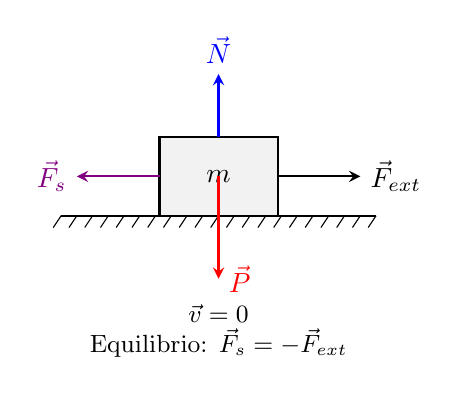
\begin{tikzpicture}[>=stealth, scale=1]
        % Piano
        \draw[thick] (-2,0) -- (2,0);
        \foreach \x in {-2,-1.8,...,2} \draw (\x,0) -- (\x-0.1,-0.15);
        
        % Corpo
        \draw[thick, fill=gray!10] (-0.75,0) rectangle (0.75,1);
        \node at (0,0.5) {$m$};
        
        % Forze
        \draw[->, thick, blue] (0,1) -- (0,1.8) node[above] {$\vec{N}$};
        \draw[->, thick, red] (0,0.5) -- (0,-0.8) node[right] {$\vec{P}$};
        
        \draw[->, thick, black] (0.75,0.5) -- (1.8,0.5) node[right] {$\vec{F}_{ext}$};
        \draw[->, thick, violet] (-0.75,0.5) -- (-1.8,0.5) node[left] {$\vec{F}_s$};
        
        \node[below, align=center, font=\small] at (0,-1) {$\vec{v} = 0$\\Equilibrio: $\vec{F}_s = - \vec{F}_{ext}$};
    \end{tikzpicture}
    \caption{Attrito Statico: si oppone alla forza motrice finché il corpo è fermo.}
\end{figure}

\subsubsection{Attrito Dinamico ($F_d$)}
È la forza parallela alla superficie presente quando il corpo è \textbf{in moto} relativo su una superficie scabra.
Si oppone sempre al versore della velocità istantanea $\hat{v}$.

A differenza dell'attrito statico, l'attrito dinamico ha un modulo (approssimativamente) \textbf{costante} durante il moto, indipendentemente dalla velocità:

\begin{equation}
    |\vec{F}_d| = \mu_d |\vec{N}|
\end{equation}

In forma vettoriale:
\begin{equation}
    \vec{F}_d = - \mu_d |\vec{N}| \cdot \hat{v}
\end{equation}

Dove:
\begin{itemize}
    \item $\mu_d$ è il \textbf{Coefficiente di Attrito Dinamico} (solitamente $\mu_d < \mu_s$).
    \item Il segno meno unito al versore $\hat{v}$ indica che il verso di $\vec{F}_d$ è sempre \textbf{opposto} a quello del moto (della velocità e dello spostamento elementare).
    \item \textbf{Nota Bene}: È SBAGLIATO scrivere $\vec{F}_d = -\mu_d \vec{N}$, poiché $\vec{F}_d$ (parallela al piano) e $\vec{N}$ (perpendicolare) sono vettori ortogonali! La relazione vettoriale corretta lega attrito e velocità, non attrito e normale.
\end{itemize}

\begin{figure}[h!]
    \centering
    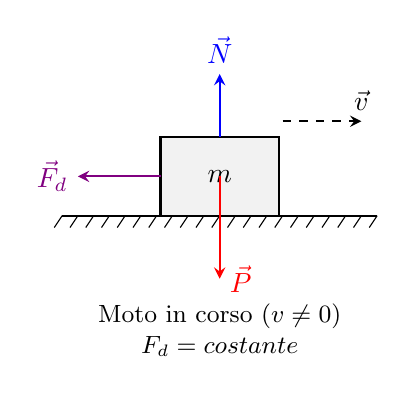
\begin{tikzpicture}[>=stealth, scale=1]
        % Piano
        \draw[thick] (-2,0) -- (2,0);
        \foreach \x in {-2,-1.8,...,2} \draw (\x,0) -- (\x-0.1,-0.15);
        
        % Corpo
        \draw[thick, fill=gray!10] (-0.75,0) rectangle (0.75,1);
        \node at (0,0.5) {$m$};
        
        % Velocità
        \draw[->, dashed, thick, black] (0.8, 1.2) -- (1.8, 1.2) node[above] {$\vec{v}$};
        
        % Forze
        \draw[->, thick, blue] (0,1) -- (0,1.8) node[above] {$\vec{N}$};
        \draw[->, thick, red] (0,0.5) -- (0,-0.8) node[right] {$\vec{P}$};
        
        \draw[->, thick, violet] (-0.75,0.5) -- (-1.8,0.5) node[left] {$\vec{F}_d$};
        
        \node[below, align=center, font=\small] at (0,-1) {Moto in corso ($v \neq 0$)\\$F_d = \text{costante}$};
    \end{tikzpicture}
    \caption{Attrito Dinamico: si oppone alla velocità del corpo.}
\end{figure}
